\documentclass{if-beamer}

% --------------------------------------------------- %
%                  Presentation info	              %
% --------------------------------------------------- %
\title[Lecture 13]{Lecture 13}
\subtitle{C++ Libraries and Classes}
\author{Instructor: Ashley Gannon}
\date{ISC3313 Fall 2021}
\logo{

\includegraphics[scale=0.08]{figures/FSULogo.png}
}
\subject{Presentation subject}

% --------------------------------------------------- %
%                    Title + Schedule                 %
% --------------------------------------------------- %
\begin{document}

\begin{frame}
  \titlepage
\end{frame}
% --------------------------------------------------- %
%                      Presentation                   %
% --------------------------------------------------- %
\section{Motivation}

\begin{frame}
\frametitle{Motivation}
\begin{itemize}
	\item In Computational Science, you will often come into contact with problems that can be solved with the algorithms covered in this course. So far we have discussed and implemented root finding algorithms, we still have to cover algorithms for\\\vspace{0.2cm}
	\begin{itemize}
		\item Optimization
		\item Integration and differentiation
		\item Ordinary Differential Equations (ODEs) \\\vspace{0.2cm}
	\end{itemize}	

\end{itemize}
\end{frame}

\begin{frame}
	\frametitle{Motivation}
	\begin{itemize}
		\item In Computational Science, you will often come into contact with problems that can be solved with the algorithms covered in this course. So far we have discussed and implemented root finding algorithms, we still have to cover algorithms for \\\vspace{0.2cm}
		\begin{itemize}
			\item Optimization
			\item Integration and differentiation
			\item Ordinary Differential Equations (ODEs) \\\vspace{0.2cm}
		\end{itemize}	
		\item Oftentimes you will use several of these algorithms together to solve one problem. \\\vspace{0.2cm}

	\end{itemize}
\end{frame}

\begin{frame}
	\frametitle{Motivation}
	\begin{itemize}
		\item In Computational Science, you will often come into contact with problems that can be solved with the algorithms covered in this course. So far we have discussed and implemented root finding algorithms, we still have to cover algorithms for \\\vspace{0.2cm}
		\begin{itemize}
			\item Optimization
			\item Integration and differentiation
			\item Ordinary Differential Equations (ODEs) \\\vspace{0.2cm}
		\end{itemize}	
		\item Oftentimes you will use several of these algorithms together to solve one problem. \\\vspace{0.2cm}
		\item If we continue to write the algorithms the way we have been, we will have to copy and paste our functions over and over again into new .cpp files so that our \texttt{main()} can call them. \\\vspace{0.2cm}
	\end{itemize}
\end{frame}


\begin{frame}
	\frametitle{Motivation}
	\begin{itemize}
		\item In Computational Science, you will often come into contact with problems that can be solved with the algorithms covered in this course. So far we have discussed and implemented root finding algorithms, we still have to cover algorithms for \\\vspace{0.2cm}
		\begin{itemize}
			\item Optimization
			\item Integration and differentiation
			\item Ordinary Differential Equations (ODEs) \\\vspace{0.2cm}
		\end{itemize}	
		\item Oftentimes you will use several of these algorithms together to solve one problem. \\\vspace{0.2cm}
		\item If we continue to write the algorithms the way we have been, we will have to copy and paste our functions over and over again into new .cpp files so that our \texttt{main()} can call them. \\\vspace{0.2cm}
		\item Wouldn't it be nice to keep all our algorithms in one place, that we can access from the \texttt{main()}, without having to copy and paste them every time? \\
	\end{itemize}
\end{frame}

\section{Libraries}

\begin{frame}
	\frametitle{Libraries}
	
	A \textbf{library} is a package of code that is meant to be reused by many programs. Typically, a C++ library comes in two pieces: \\\vspace{0.2cm}
	\begin{enumerate}
		\item A header file that defines the functionality the library is offering to the programs using it.
		\item A precompiled .cpp file that contains the implementation of that functionality.\\\vspace{0.2cm}
	\end{enumerate}
	We've used a few libraries already:\\\vspace{0.2cm}
	\begin{itemize}
		\item \texttt{stdio}
		\item \texttt{iostream}
		\item \texttt{iomanip}
		\item \texttt{cmath} \\\vspace{0.2cm}
	\end{itemize}
	There are two types of libraries: \textbf{static libraries} and \textbf{dynamic libraries}.	We will likely only cover static libraries in this course.
\end{frame}

\begin{frame}
	\frametitle{Libraries}
	\begin{itemize}
		\item A static library consists of routines that are compiled and linked directly into your program. \\\vspace{0.2cm}
		\begin{itemize}
			\item Namespaces
			\item Classes
			\item Functions
		\end{itemize}
		\item When you compile a program that uses a static library, all the functionality of the static library that your program uses becomes part of your executable.\\\vspace{0.2cm}
		\begin{itemize}
			\item On Windows, static libraries typically have a \texttt{.lib} extension
			\item On linux, static libraries typically have an \texttt{.a} extension.\\\vspace{0.2cm}
		\end{itemize}
		NOTE: We will be using visual studio to write our library, so everyone should end up with a \texttt{.lib} extension. 
	\end{itemize}	
\end{frame}

\begin{frame}
    \frametitle{Example}
	The purpose of this course is to introduce you all to standard problems in computational science, as well as the basics of C++ -- with the intention of facilitating the student’s implementation of algorithms. So I won't go into the gritty details of this.
	\begin{figure}
		\centering
		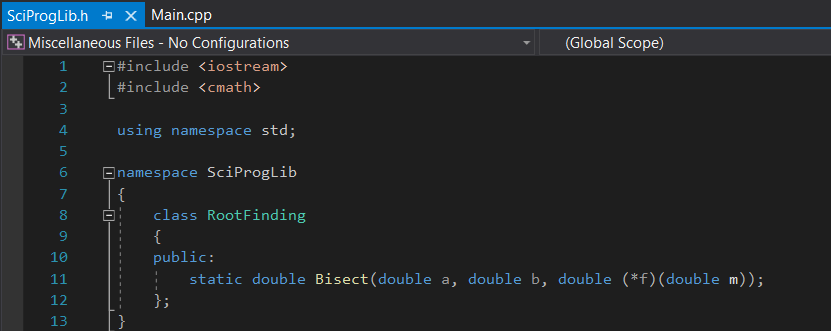
\includegraphics[width = \textwidth]{figures/headerfile}
	\end{figure}
\end{frame}

\begin{frame}
	\frametitle{Example}
	The purpose of this course is to introduce you all to standard problems in computational science, as well as the basics of C++ -- with the intention of facilitating your implementation of the algorithms we cover. So I won't go into the gritty details of this. If you would like more details, come see me or Liam during office hours.
	\begin{figure}
		\centering
		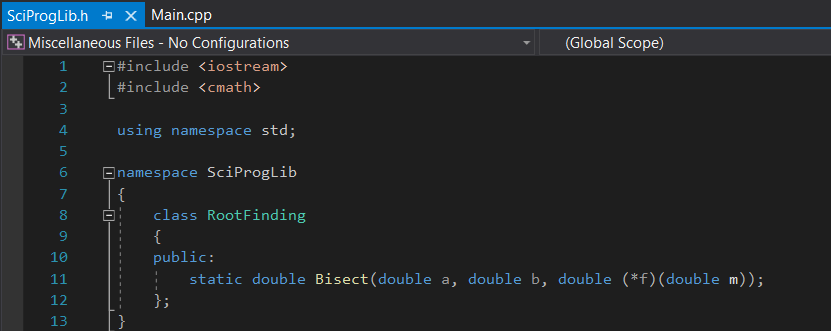
\includegraphics[width = \textwidth]{figures/headerfile}
	\end{figure}
\end{frame}

\begin{frame}
	\frametitle{Example}
	Say we want our friend “Bisect" to help with our homework. We’ll need to know how to get over to his place. We know that he lives in the “SciProgLib” neighborhood, on the “SciProgLib” street in the “RootFinding” house.
	\begin{figure}
		\centering
		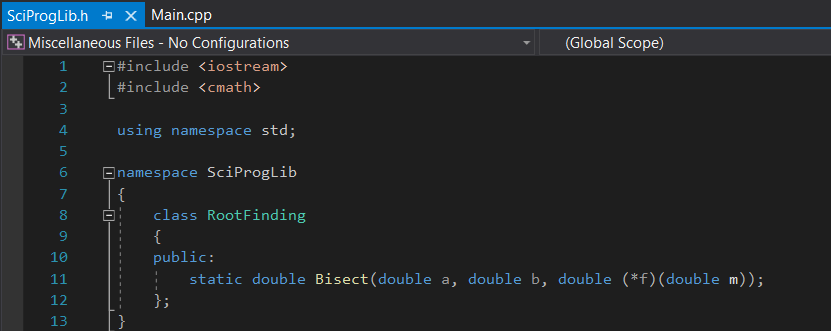
\includegraphics[width = \textwidth]{figures/headerfile}
	\end{figure}
\end{frame}

\begin{frame}
	\frametitle{Example}
	The neighborhood would be the header file, \\
	the street would be the namespace, \\
	and the house would be the class, \\
	and right now, think of Bisect as a person who lives in the house alone.
	\begin{figure}
		\centering
		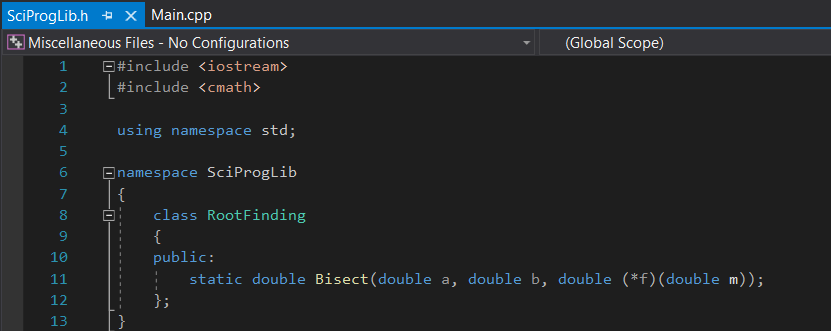
\includegraphics[width = \textwidth]{figures/headerfile}
	\end{figure}
\end{frame}

\begin{frame}
	\frametitle{Example}
	A class is a data structure that can contain a data member or a function member. In this example, our class \texttt{RootFinding} contains the function member \texttt{Bisect}. 
	\begin{figure}
		\centering
		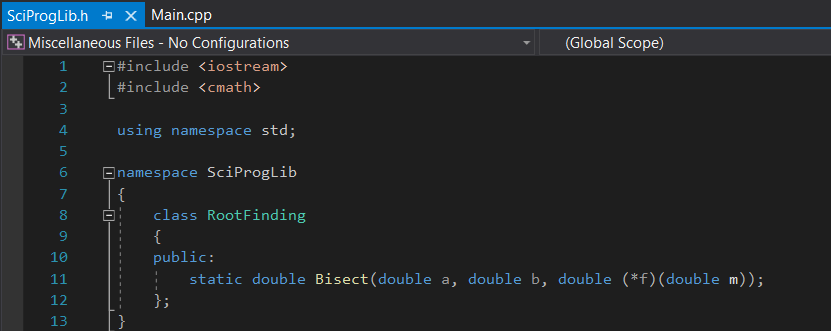
\includegraphics[width = \textwidth]{figures/headerfile}
	\end{figure}
\end{frame}

\begin{frame}
	\frametitle{Example}
	Classes also contain something called an \textit{access specifier}, which can be \texttt{public}, \texttt{private}, or \texttt{protected}. These specifiers modify the access rights for the members that follow them. In this case, thinking back to our simple example, because our class is \texttt{public} “Bisect” helps everyone with homework. But if he was \texttt{private}, he would only help people who live in the same house as him. 
	\begin{figure}
		\centering
		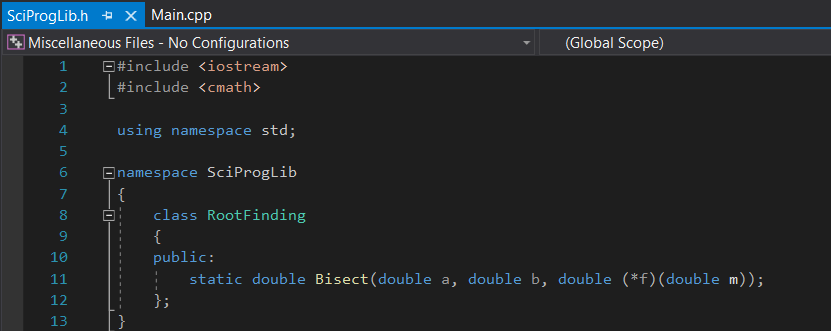
\includegraphics[width = \textwidth]{figures/headerfile}
	\end{figure}
\end{frame}

\begin{frame}
	\begin{minipage}{0.5\textwidth}
		\frametitle{Example}
		\begin{figure}
			\centering
			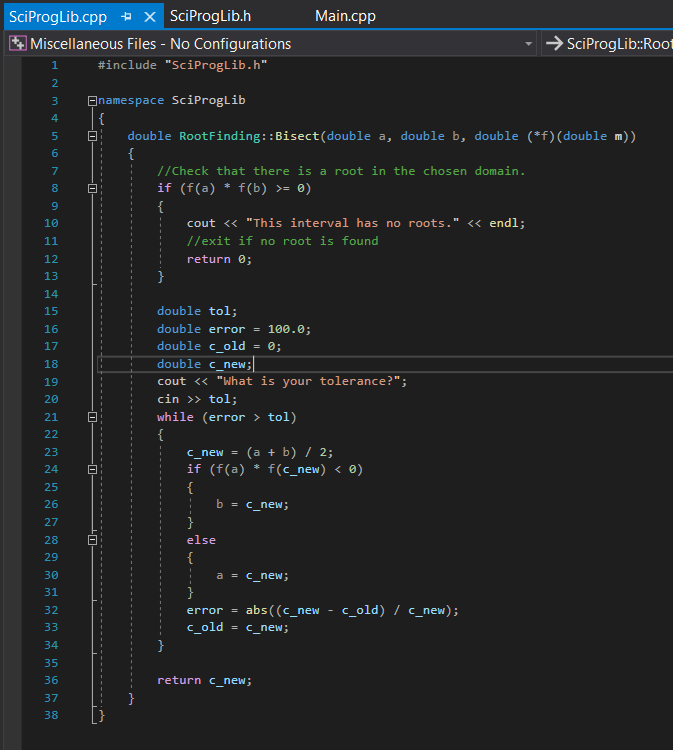
\includegraphics[width = \textwidth]{figures/cppfile}
		\end{figure}
	\end{minipage}
	\begin{minipage}{0.5\textwidth}
		Now we can use SciProgLib in another .cpp file. We \texttt{\#include} the header file so that the compiler pulls in the declaration of the member function \texttt{Bisect}. All the compiler needs to know is that \texttt{RootFinding} is a class that has a public member function called \texttt{Bisect}.
	\end{minipage}
	
\end{frame}

\begin{frame}
	\frametitle{Example}
	Now when we include our header file \texttt{"SciProgLib."} in the same .cpp file as our \texttt{main()}, we are able to call the \texttt{Bisect} function.
		\begin{figure}
		\centering
		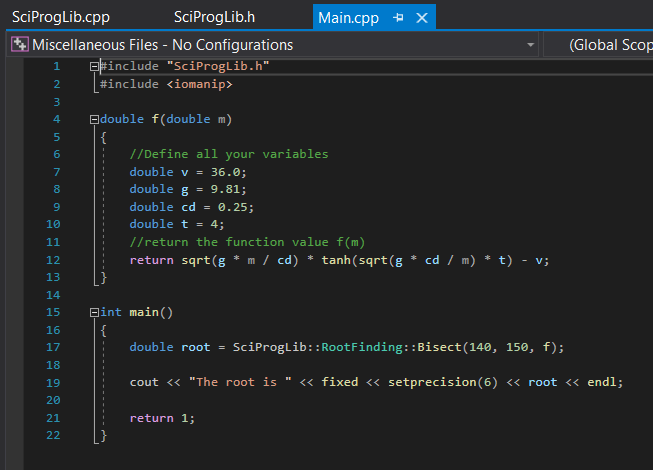
\includegraphics[width = .7\textwidth]{figures/main}
	\end{figure}
\end{frame}


\begin{frame}
	\frametitle{Example}
	In this example, note that we are also passing in a pointer of the function f that we use in the \texttt{Bisect} function. This is useful in the sense that we don't have to define the function in the same space as \texttt{Bisect}, and recompile our library every time we change it.
	\begin{figure}
		\centering
		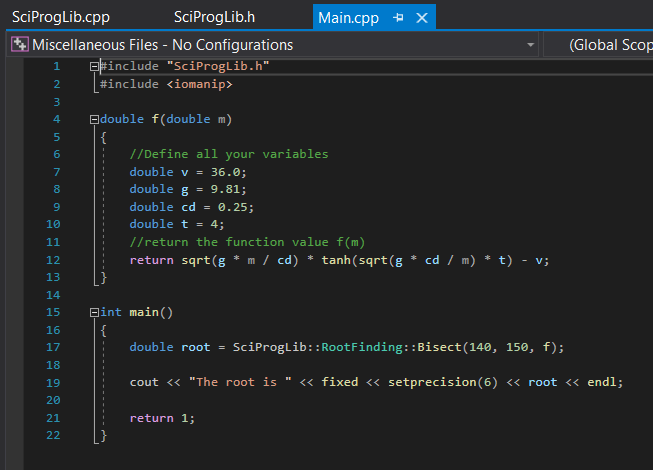
\includegraphics[width = .7\textwidth]{figures/main}
	\end{figure}
\end{frame}

\begin{frame}
	\frametitle{Mini Assignment}
	We will take the remainder of the class period (and any extra time you need) to create a new project in visual studio that builds this library. 
	\\\vspace{0.5cm}
	Submit your project as a \textbf{.zip} file to canvas. If you are having trouble generating a .zip file, please see these instructions: \\ https://www.hellotech.com/guide/for/how-to-zip-a-file-mac-windows-pc \\\vspace{0.5cm}
	\textbf{Due by the start of next class.}
	
\end{frame}	

\end{document}
